\documentclass[coursework]{SCWorks}
% Тип обучения (одно из значений):
%    bachelor   - бакалавриат (по умолчанию)
%    spec       - специальность
%    master     - магистратура
% Форма обучения (одно из значений):
%    och        - очное (по умолчанию)
%    zaoch      - заочное
% Тип работы (одно из значений):
%    coursework - курсовая работа (по умолчанию)
%    referat    - реферат
%  * otchet     - универсальный отчет
%  * nirjournal - журнал НИР
%  * digital    - итоговая работа для цифровой кафедры
%    diploma    - дипломная работа
%    pract      - отчет о научно-исследовательской работе
%    autoref    - автореферат выпускной работы
%    assignment - задание на выпускную квалификационную работу
%    review     - отзыв руководителя
%    critique   - рецензия на выпускную работу

% * Добавлены вручную. За вопросами к @mchernigin
\usepackage{preamble}

\begin{document}

% Кафедра (в родительном падеже)
\chair{математической кибернетики и компьютерных наук}

% Тема работы
\title{Линейная регрессия и метод градиентного спуска}

% Курс
\course{3}

% Группа
\group{351}

% Факультет (в родительном падеже) (по умолчанию "факультета КНиИТ")
% \department{факультета КНиИТ}

% Специальность/направление код - наименование
% \napravlenie{02.03.02 "--- Фундаментальная информатика и информационные технологии}
% \napravlenie{02.03.01 "--- Математическое обеспечение и администрирование информационных систем}
% \napravlenie{09.03.01 "--- Информатика и вычислительная техника}
\napravlenie{09.03.04 "--- Программная инженерия}
% \napravlenie{10.05.01 "--- Компьютерная безопасность}

% Для студентки. Для работы студента следующая команда не нужна.
% \studentfemale

% Фамилия, имя, отчество в родительном падеже
\author{Рзаева Амира Абилевича}

% Заведующий кафедрой 
\chtitle{доцент, к.\,ф.-м.\,н.}
\chname{С.\,В.\,Миронов}

% Руководитель ДПП ПП для цифровой кафедры (перекрывает заведующего кафедры)
% \chpretitle{
%     заведующий кафедрой математических основ информатики и олимпиадного\\
%     программирования на базе МАОУ <<Ф"=Т лицей №1>>
% }
% \chtitle{г. Саратов, к.\,ф.-м.\,н., доцент}
% \chname{Кондратова\, Ю.\,Н.}

% Научный руководитель (для реферата преподаватель проверяющий работу)
\satitle{доцент, к.\,ф.-м.\,н.} %должность, степень, звание
\saname{А.\,Д.\,Панфёров}

% Руководитель практики от организации (руководитель для цифровой кафедры)
\patitle{доцент, к.\,ф.-м.\,н.}
\paname{С.\,В.\,Миронов}

% Руководитель НИР
\nirtitle{доцент, к.\,п.\,н.} % степень, звание
\nirname{В.\,А.\,Векслер}

% Семестр (только для практики, для остальных типов работ не используется)
\term{2}

% Наименование практики (только для практики, для остальных типов работ не
% используется)
\practtype{учебная}

% Продолжительность практики (количество недель) (только для практики, для
% остальных типов работ не используется)
\duration{2}

% Даты начала и окончания практики (только для практики, для остальных типов
% работ не используется)
\practStart{01.07.2024}
\practFinish{13.01.2024}

% Год выполнения отчета
\date{2026}

\maketitle

% Включение нумерации рисунков, формул и таблиц по разделам (по умолчанию -
% нумерация сквозная) (допускается оба вида нумерации)
\secNumbering

\tableofcontents

% Раздел "Обозначения и сокращения". Может отсутствовать в работе
% \abbreviations
% \begin{description}
%     \item ... "--- ...
%     \item ... "--- ...
% \end{description}

% Раздел "Определения". Может отсутствовать в работе
% \definitions

% Раздел "Определения, обозначения и сокращения". Может отсутствовать в работе.
% Если присутствует, то заменяет собой разделы "Обозначения и сокращения" и
% "Определения"
% \defabbr

\intro
Линейная регрессия "--- одна из базовых моделей машинного обучения, на примере которой удобно разбирать общие принципы подбора параметров по данным \cite{ESL,PRML}. Параметры модели можно найти аналитически, но на больших выборках и для более сложных моделей используют итерационные методы оптимизации, прежде всего градиентный спуск, стохастические варианты которого восходят к работе Роббинса и Монро \cite{RobbinsMonro}.

Цель работы "--- сравнить аналитическое решение задачи линейной регрессии с решением методом градиентного спуска. Для этого необходимо:
\begin{itemize}
    \item записать модель и функцию потерь;
    \item реализовать оба метода на языках Python и C++;
    \item исследовать влияние шага обучения на сходимость метода.
\end{itemize}

\section{Теоретическая часть}
\subsection{Модель и функция потерь}
Рассматривается выборка из $n$ пар $(x_i, y_i)$. Модель линейной регрессии предсказывает значение
\begin{equation}
    \hat{y}_i = \omega x_i + b,
    \label{eq:model}
\end{equation}
где $\omega$ "--- коэффициент наклона (в коде \texttt{w}), $b$ "--- свободный член (в коде
\texttt{b}). Качество модели оценивается средним квадратом ошибки:
\begin{equation}
    L(\omega,b) = \frac{1}{n}\sum\limits_{i=1}^n(\omega x_i + b - y_i)^2.
    \label{eq:mse}
\end{equation}

\subsection{Аналитическое решение}
Минимум функции $L$ достигается в точке, где обращается в нуль градиент.
Обозначим $X$ "--- матрицу размера $n \times 2$, первый столбец которой составлен
из $x_i$, а второй "--- из единиц, и $\theta = (\omega, b)^T$. Тогда решение нормального
уравнения имеет вид
\begin{equation}
    \theta = (X^TX)^{-1}X^Ty.
    \label{eq:normal}
\end{equation}
\subsection{Градиентный спуск}
Частные производные функции потерь равны
\begin{equation}
    \frac{\partial L}{\partial \omega} = \frac{2}{n}\sum\limits_{i=1}^n(\hat{y}_i-y_i)x_i,
    \quad
    \frac{\partial L}{\partial b} = \frac{2}{n} \sum\limits_{i=1}^n(\hat{y}_i-y_i).
    \label{eq:grad}
\end{equation}
На каждой итерации параметры сдвигаются в сторону антиградиента:
\begin{equation}
    \omega \leftarrow \omega - \alpha \frac {\partial L}{\partial \omega},
    \quad
    b \leftarrow b - \alpha \frac {\partial L}{\partial b},
    \label{eq:update}
\end{equation}
где $\alpha > 0$ "--- шаг обучения. Для квадратичной функции $L$ с матрицей
вторых производных $H = \frac{2}{n}X^T X$ метод сходится при
\begin{equation}
    \alpha < \frac{2}{\lambda_{\max}(H)},
    \label{eq:stability}
\end{equation}
где $\lambda_{\max}(H)$ "--- наибольшее собственное значение матрицы $H$ \cite{DeepLearning}.

\section{Практическая часть}

\subsection{Данные и реализация}

Для эксперимента сгенерирована выборка из 50 точек. Значения $x_i$ равномерно распределены на отрезке $[0;\,10]$, а отклики вычисляются по формуле $y_i = 2{,}5\,x_i + 1 + \varepsilon_i$, где $\varepsilon_i$ "--- нормальный шум со стандартным отклонением $1{,}5$. Истинные параметры, уровень шума и начальное значение генератора случайных чисел задаются аргументами \texttt{w\_true}, \texttt{b\_true}, \texttt{noise} и \texttt{seed=42} функции \mintinline{python}{generate_data}, поэтому эксперимент воспроизводим. Расчёты выполнены с помощью библиотеки NumPy~\cite{numpy}.

Программа на Python содержит четыре функции:
\begin{itemize}
\item \texttt{mse} вычисляет значение функции потерь~\eqref{eq:mse};
\item \texttt{normal\_equation} находит параметры по формуле~\eqref{eq:normal};
\item \texttt{gradient\_descent} выполняет итерации по правилу~\eqref{eq:update}, используя градиенты~\eqref{eq:grad} (переменные \texttt{grad\_w} и \texttt{grad\_b});
\item \texttt{generate\_data} создаёт выборку.
\end{itemize}
Шаг обучения передаётся в \texttt{gradient\_descent} аргументом \texttt{learning\_rate}, число итераций "--- аргументом \texttt{epochs} (по умолчанию 1000). Полный текст программы приведён в приложении~\ref{app:python}.

Тот же шаг градиентного спуска, реализованный на C++, показан в листинге~\ref{code:cpp-step}: функция \texttt{gradient\_step} принимает модель \texttt{model}, векторы \texttt{x} и \texttt{y} и шаг \texttt{learning\_rate}, вычисляет градиенты~\eqref{eq:grad} и обновляет параметры \texttt{model.w} и \texttt{model.b}.

\begin{listing}[ht]
\caption{Шаг градиентного спуска на C++}
\label{code:cpp-step}
\inputminted[firstline=9, lastline=21, firstnumber=1]{cpp}{code/gradient_step.cpp}
\end{listing}

Для проверки реализации функция запускалась на пяти точках $x = 1,\dots,5$ с откликами $3{,}6;\ 6{,}1;\ 8{,}4;\ 11{,}1;\ 13{,}4$ (2000 итераций, шаг $0{,}02$). Программа вывела \texttt{w = 2.46, b = 1.14}. Эти значения совпадают с решением нормального уравнения~\eqref{eq:normal} для тех же точек.

\subsection{Результаты}

На рис.~\ref{fig:fit} показаны исходные данные и прямая, найденная по формуле нормального уравнения~\eqref{eq:normal}: $y = 2{,}52x + 0{,}65$. Коэффициент детерминации равен $R^2 = 0{,}974$, то есть модель объясняет почти всю изменчивость откликов. Найденные коэффициенты близки к истинным $\omega = 2{,}5$ и $b = 1$; отклонение свободного члена объясняется шумом в данных.

\begin{figure}[H]
\centering
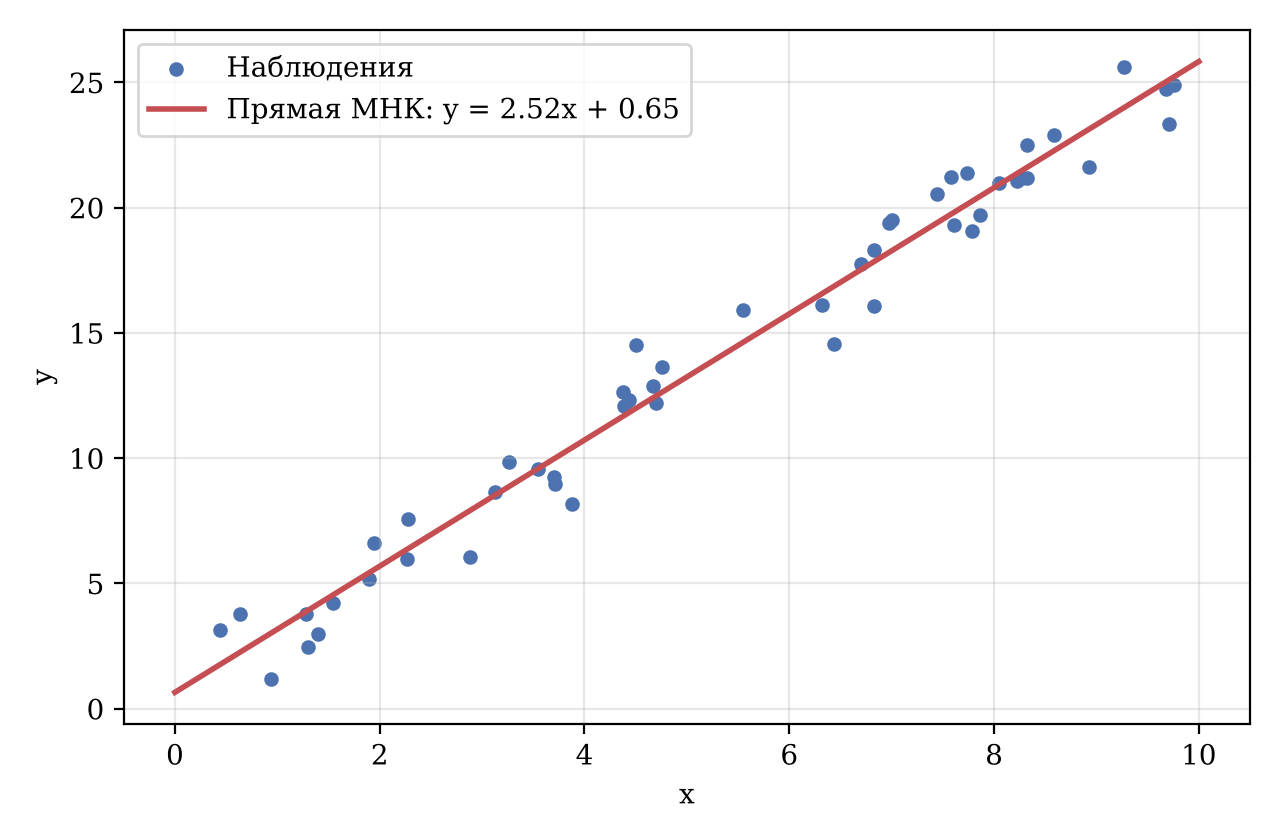
\includegraphics[width=0.75\textwidth]{images/regression_fit.png}
\caption{Данные и регрессионная прямая}
\label{fig:fit}
\end{figure}

Динамика ошибки при разных значениях шага обучения показана на рис.~\ref{fig:loss}, а итоговые значения параметров "--- в таблице~\ref{tab:results}. Чем больше $\alpha$, тем быстрее убывает $L$. Так, значение, не превышающее $1{,}01\cdot\min L$, достигается за 257 итераций при $\alpha = 0{,}001$, за 52 при $\alpha = 0{,}005$ и всего за 26 при $\alpha = 0{,}01$.

\begin{figure}[H]
\centering
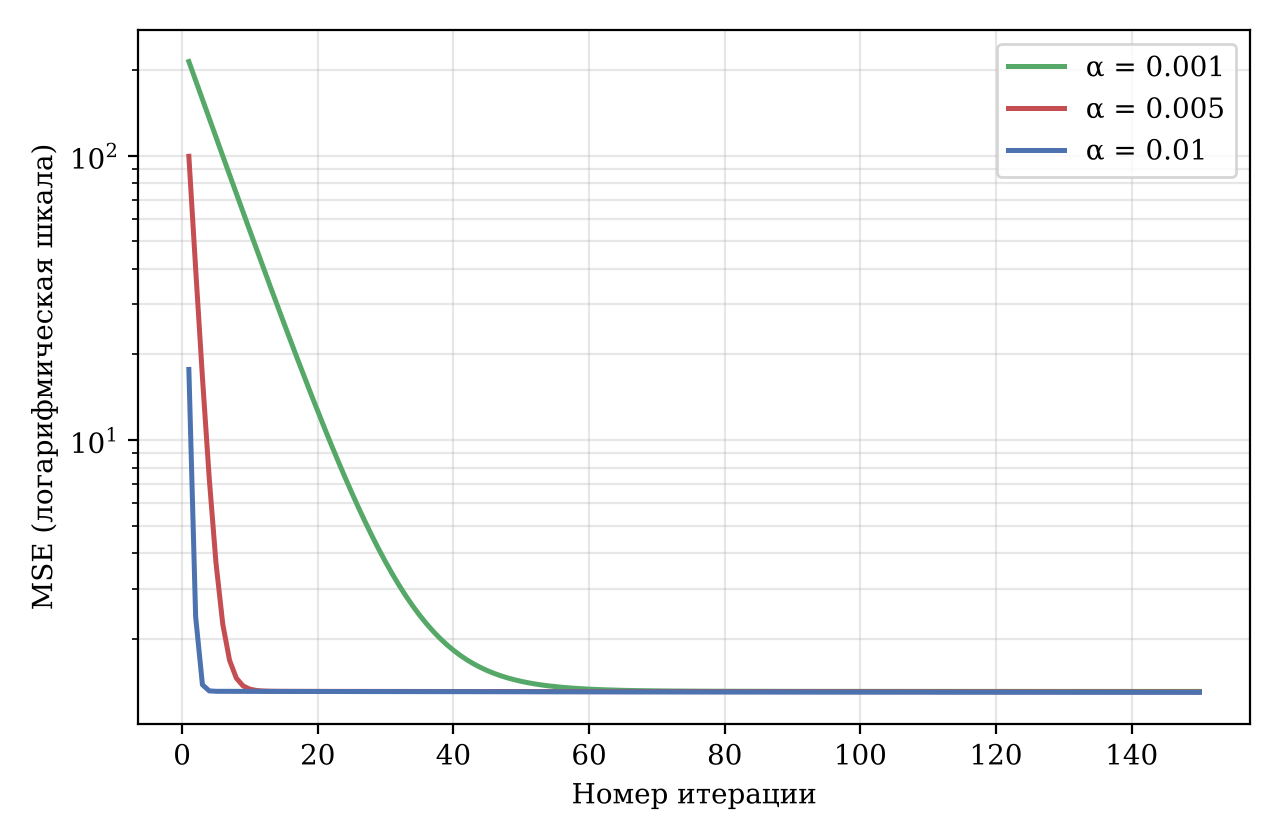
\includegraphics[width=0.75\textwidth]{images/loss_curves.png}
\caption{Зависимость ошибки MSE от номера итерации}
\label{fig:loss}
\end{figure}

\begin{table}[H]
\caption{Сравнение методов (1000 итераций градиентного спуска)}
\label{tab:results}
\centering
\small
\begin{tabular}{|p{5.6cm}|c|c|c|>{\centering\arraybackslash}p{3.2cm}|}
\hline
Метод & $\omega$ & $b$ & MSE & Итераций до $1{,}01\cdot\min L$ \\
\hline
Нормальное уравнение & 2,5181 & 0,6530 & 1,2903 & --- \\
\hline
Градиентный спуск, $\alpha=0{,}001$ & 2,5449 & 0,4720 & 1,2973 & 257 \\
\hline
Градиентный спуск, $\alpha=0{,}005$ & 2,5232 & 0,6187 & 1,2906 & 52 \\
\hline
Градиентный спуск, $\alpha=0{,}01$ & 2,5187 & 0,6487 & 1,2903 & 26 \\
\hline
\end{tabular}
\end{table}

Из таблицы~\ref{tab:results} видно, что при $\alpha = 0{,}01$ градиентный спуск практически совпадает с аналитическим решением: коэффициент $\omega$ отличается от точного менее чем на $10^{-3}$, свободный член $b$ "--- примерно на $0{,}004$, а значения MSE совпадают до четвёртого знака. При $\alpha = 0{,}001$ за 1000 итераций метод ещё не успевает полностью сойтись, и параметры заметно отличаются от точных.

Увеличивать шаг можно лишь до границы устойчивости. Для построенной выборки $2/\lambda_{\max}(H) \approx 0{,}0269$, поэтому при $\alpha = 0{,}03$ условие~\eqref{eq:stability} нарушается, и значения $L$ неограниченно растут. В эксперименте это проявляется как переполнение при вычислении ошибки.

\conclusion
В работе записаны модель линейной регрессии и функция потерь, оба метода подбора параметров реализованы на языках Python и C++, исследовано влияние шага обучения на сходимость градиентного спуска. Аналитическое решение и градиентный спуск дают практически одинаковые параметры модели: при $\alpha=0{,}01$ различие по коэффициенту $\omega$ не превышает $10^{-3}$. Скорость сходимости растёт с увеличением шага, но только до границы устойчивости $2/\lambda_{\max}(H)$, при превышении которой метод расходится.

% Отобразить все источники. Даже те, на которые нет ссылок.
% \nocite{*}

\bibliographystyle{ugost2003}
\bibliography{thesis}

% Окончание основного документа и начало приложений Каждая последующая секция
% документа будет являться приложением
\appendix
\section{Листинг программы на Python}
\label{app:python}

\inputminted{python}{code/gradient_descent.py}

\end{document}
